\newcommand{\rtmaude}{Real Time Maude}

\thesischapter{The Application of Real Time Maude to Model and Verify the European Rail Traffic Management System}
In the following we present the Maude \cite{MC03,Maude} and Real Time Maude \cite{PO02,PO04,RTMaude} tools and describe an approach using these tools to model and verify ERTMS \ref{}.The property we verify is that no two trains on our example railway share the same movement authority which 


\section{The European Rail Traffic Management System}

\section{Formalising the European Rail Traffic Management System Using Hybrid Automata}
One formalism which we can use to real about systems such as ERTMS is hybrid automata \cite{TH96}.

\begin{mydef}[Hybrid Automaton: Syntax]
The syntax of a hybrid automaton $H$ comprises of the following:
\begin{description}
\item[Variables] A finite set $X = \{x_1, \ldots x_n \}$ of variables which range over the real numbers. The cardinality of $|X|$ is called the \emph{dimension} of $H$. The variable set has a corresponding dotted variable set $\dot{X} = \{\dot{x}_1, \ldots \dot{x}_n \}$ which represents the continuous changes of variables and a primed variable set $X' = \{x'_1, \ldots , x'_n \}$ that represents  values at the conclusion of a discrete change.

\item[Control graph] A finite directed multigraph $(V,E)$ consisting of a set of vertices which we shall refer to as \emph{control modes} and a set of edges $E$ which we shall refer to as \emph{control switches}.

\item[Initial, invariant and flow conditions] Three functions \emph{init},\emph{inv} and \emph{flow} that label each control mode $v \in V$ with three predicates such that for all $v \in V$, $\freevar{init(v)} \subseteq X$, $\freevar{inv(v)} \subseteq \dot{X}$ and $\freevar{flow(v)} \subseteq X \cup \dot{X}$. 

\item[Jump Conditions] A function \emph{jump} that labels each edge $e \in E$ with a predicate such that $\freevar{jump(e)} \subseteq X \cup X' $.

\item[Events] A finite set $\Sigma$ of \emph{events}, at least one of which is assigned to  each control switch by a labelling function $event: E \to \Sigma$.

\end{description}
Where $\freevar{P}$ is the set of free variables in the predicate $P$.
\end{mydef}


\begin{mydef}[Labelled Transition System]
We define a \emph{labelled transition system} $LTS = (S,S_0,T,L)$ as follows:
\begin{itemize}

\item $S$ is a possibly infinite set of states

\item $S_0$ is a set of initial states $S_0 \subseteq S$

\item $L$ is a set of \emph{labels}

\item $T$ is a binary relation $\xrightarrow{a}$ over the state space $S$.

\end{itemize}
\end{mydef}

When defining the semantics of a hybrid automata we need to be able to speak about parts of the state space.  We define a \emph{region} as being a subset of the state space $R \subseteq S$.

\begin{mydef}[Transition Semantics of Hybrid Automata]
We define the semantics of a hybrid automaton $H$ in terms of a \emph{timed transition system} $LTS^t_H = (S,S_0,L,T)$ as follows:


\begin{itemize}
 
\item The state space $S$ of the timed transition system is defined as, $S, S_0 \subseteq V \times R^n$. A state is in the state space $(v,x) \in S_0$ iff the closed predicate $inv(v)[X := x]$ holds. In addition to the previous condition a state is in the initial state space $(v,x) \in S_0$ iff the closed predicate $init(v)[X := x]]$ holds. We call a subset of the state space $S$ a \emph{H-region}.


\item $L = \Sigma \cup R_{\geq 0}$

\item For all events $\sigma \in \Sigma$ such that there exists a control switch $e \in E$, define $(v,x) \xrightarrow{\sigma} (v',x')$ iif the following conditions are satisified:
\begin{enumerate}
\item the source and target of $e$ are $v$ and $v'$ respectively. 
\item the closed predicate $jump(e)[X, X' := x,x']$ holds.
\item $event(e) = \sigma$.
\end{enumerate}

\item blah
\end{itemize}


\end{mydef}

The following is a simple example railway we shall use for the purposes of demonstrating our verification approach.  It contains 5 track segments connected to form a pentagon with two trains. This captures most of the behaviours found in a larger more complicated railway as the trains and control systems view any piece of track as a set of track segments joined together to form a route.

\begin{figure} [h!]

\begin{center}
\begin{tikzpicture}[node distance = 3cm]


\node (A) [draw,regular polygon, regular polygon sides=5, minimum size=6 cm,outer sep=0pt] {};
\foreach \n in {1,...,5} {

    \pgfmathtruncatemacro{\value}{(\n - 1) * 50};
    \node at (A.corner \n) [anchor=360/5*(\n-1)+270] {D = \value};
    \node at (A.side \n) [anchor = 360/5 *(\n-1) +270] {$t_{\n}$};
}

\node (B) [draw, rectangle, rotate = 36] at (-1.9,2.6) {Train A};
\node (C) [draw, rectangle, rotate =72] at (3,-1) {Train B};

\end{tikzpicture} 
\end{center}

\label{fig:trackplan}
 \caption{Pentagon Example}
\end{figure}

\begin{comment}



\def\r{3} 
\def\sone{ \sin 32}
\def\stwo{\sin 72}
\def\cone{\cos 32}
\def\ctwo{\cos 72}
\coordinate(top) at (0,\r);
\coordinate(topleft) at ({ \r * -cos (36)},{ \r * -sin (36)});
\coordinate(topright) at ({ \r * cos (72)}, { \r * -sin (72)});
\coordinate(botleft) at ({ \r * - cos (36)},{ \r * sin (36)});
\coordinate(botright) at ({\r * sin (72)},{\r * cos (72)});

\tikzstyle{box1}=[circle, draw, text width = 2cm, font=\scriptsize]
\tikzstyle{box3}=[rectangle, draw, text width = 2cm, font=\scriptsize]
\tikzstyle{arrow}=[->, thick]
\tikzstyle{biarrow}=[<->,very thick,shorten >=7pt,shorten <=7pt]


\node (A) [font = \scriptsize]  at (topleft)                  {D =150 };

\node (B) [font = \scriptsize]    at (botleft)          {D = 0};

\node (C)[font = \scriptsize] at (top)  { D = 100
						};

\node (D)[font = \scriptsize] at (botright)  { D = 50
						};

\node (E) [font = \scriptsize] at (topright) {D = 200};

\draw [arrow] (D) -- node[right] {$t_1$} (E);
\draw [arrow] (A) -- node[below = 10pt] {$t_4$} (B);
\draw [arrow] (B) --  node[above = 10pt] {$t_2$} (C);
\draw [arrow] (C) -- node [left] {$t_3$} (D);
\end{comment}
We have modelled the ETMS system controlling the pentagon example (see fig \ref{fig:trackplan}) using several hybrid automata. In this example the value $D(t)$ represents the distance from the start point at time $t$. 
It contains 2 trains $A$ and $B$ and 5 track circuits $l_0, \ldots , l_4$. The track is uni-directional allowing trains to travel from $0 - 249$. 


\begin{figure} [h!]

\begin{center}
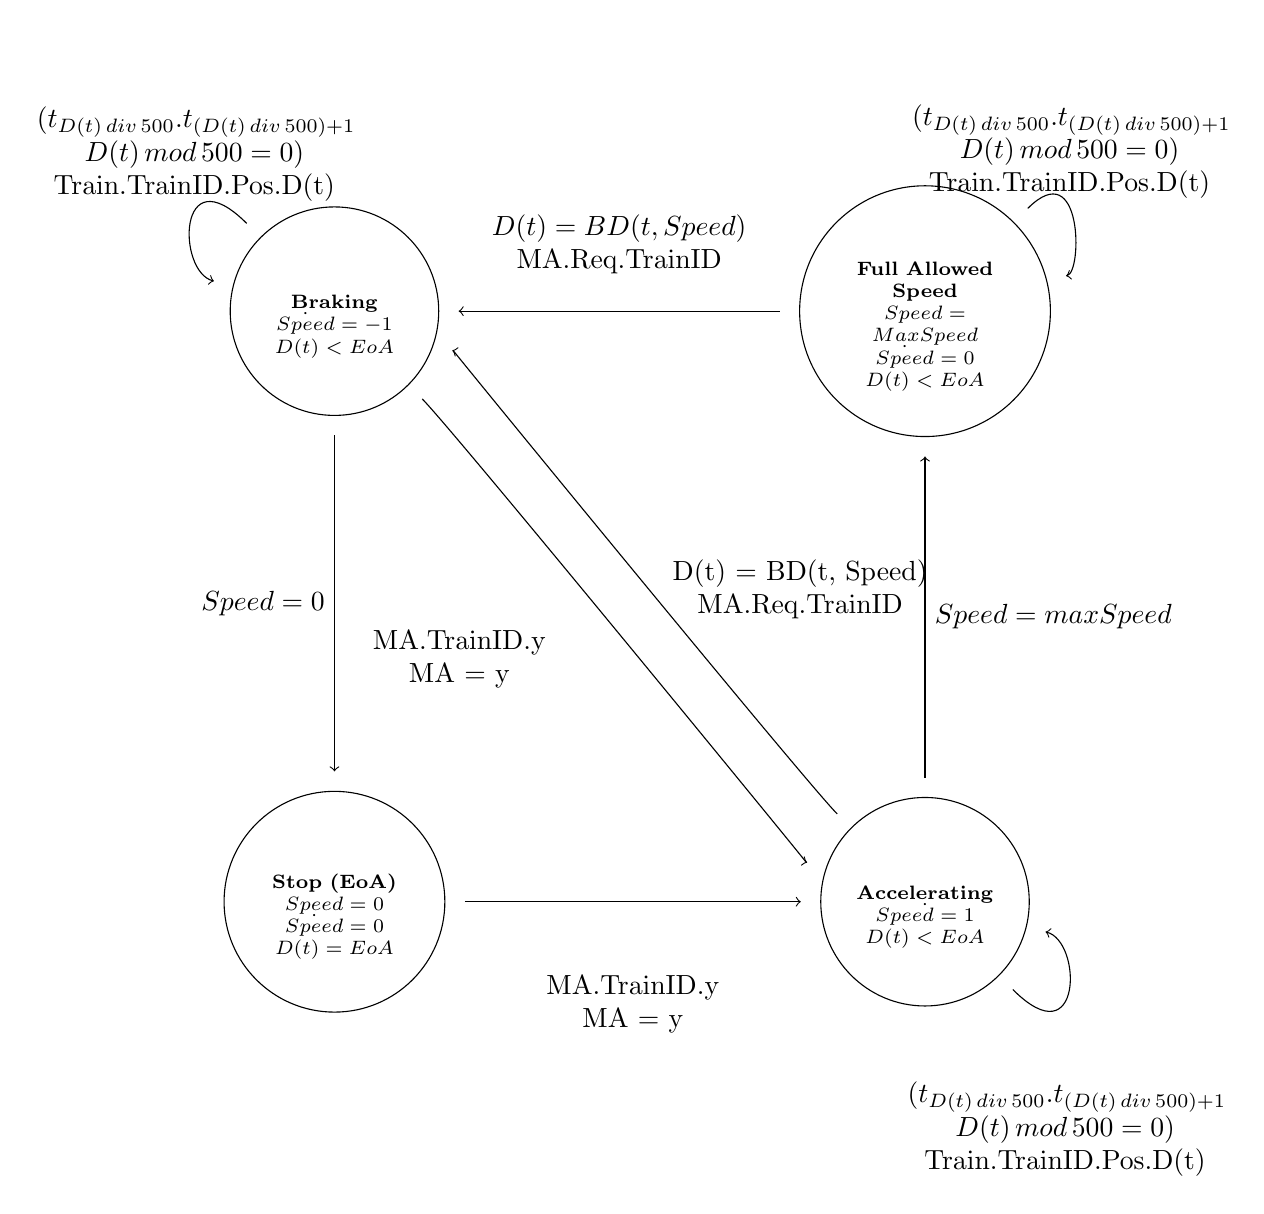
\begin{tikzpicture}[node distance = 2cm]

\tikzstyle{box1}=[circle, draw, text width = 2cm, font=\scriptsize]
\tikzstyle{box3}=[rectangle, draw, text width = 2cm, font=\scriptsize]
\tikzstyle{arrow}=[->,shorten >=7pt,shorten <= 7pt]
\tikzstyle{biarrow}=[<->,very thick,shorten >=7pt,shorten <=7pt]


\node (A) [box1]  at (0,0)                  {\begin{center} \textbf{Stop (EoA)} \\
							$Speed = 0$
                                                        $\dot{Speed} = 0$
							$D(t) = EoA$  \end{center}

                                            };

\node (B) [box1]    at (7.5,0)          {\begin{center} \textbf{Accelerating} \\
       $\dot{Speed = 1}$
       $D(t) < EoA$  \end{center}

};

\node (C)[box1] at (0, 7.5)  { \begin{center} \textbf{Braking}\\
					                   $\dot{Speed} = -1$ 
						           $D(t) < EoA$\end{center}
                                               
						};

\node (D)[box1] at (7.5, 7.5)  { \begin{center} \textbf{Full Allowed Speed }\\
					                   $Speed = MaxSpeed$
                                                            $\dot{Speed} = 0$
							    $D(t) < EoA$
                                                            \end{center}
                                               
						};


\draw [arrow] (B) -- node[right] {$Speed = max Speed$} (D);
\draw [arrow] (A) -- node[below = 10pt, text width = 4cm] {\begin{center}MA.TrainID.y\\ MA = y\end{center} } (B);
\draw [arrow] (D) --  node[above = 10pt,text width=4cm] {\begin{center}$D(t) = BD(t, Speed)$\\MA.Req.TrainID \end{center}} (C);
\draw [arrow] (C) -- node [left] {$Speed = 0$} (A);
\draw [arrow] (B)  .. controls +(-1.5cm,  1.5 cm) and +(1.5cm,  -0.5 cm ) .. node [right,text width=4cm] { \begin{center}D(t) = BD(t, Speed)\\MA.Req.TrainID \end{center}} (C);
\draw [arrow] (C) .. controls +(1.5cm,  -1.5cm) and +(-1.5cm, 0.5 cm ) ..   node [left,text width = 4cm] {\begin{center}MA.TrainID.y\\ MA = y\end{center} } (B);
\draw [arrow] (C) .. controls +(-2cm,  2cm) and +(-2cm, 0.5 cm ) ..   node [above = 5pt, text width = 4cm] {\begin{center}$(t_{D(t) \, div \, 500}.t_{(D(t) \, div \, 500) +1} $\\$D(t) \, mod \, 500 = 0)$\\Train.TrainID.Pos.D(t) \end{center}} (C);
\draw [arrow] (D) .. controls +(2cm,  2cm) and +(2cm, 0.5 cm ) ..   node [above = 5pt, text width = 4cm] {\begin{center}$(t_{D(t) \, div \, 500}.t_{(D(t) \, div \, 500) +1} $\\$D(t) \, mod \, 500 = 0)$\\Train.TrainID.Pos.D(t) \end{center}} (D);
\draw [arrow] (B) .. controls +(2cm,  -2cm) and +(2cm, -0.5 cm ) ..   node [below = 6pt, text width = 4cm] {\begin{center}$(t_{D(t) \, div \, 500}.t_{(D(t) \, div \, 500) +1} $\\$D(t) \, mod \, 500 = 0)$\\Train.TrainID.Pos.D(t) \end{center}} (B);

\end{tikzpicture} 
\end{center}

\label{fig:ContactOrders}
\end{figure}




\begin{mydef}[Interlocking Hybrid Automaton]
We define a hybrid automaton $H_{IL}$ as follows:
\begin{description}
\item[Variables] The state of the interlocking automaton consists of five boolean variables  $\underbrace{l_0, \ldots , l_4}_\text{Occupied/Free}$ and a variable $ReqID$ ranging over $\{0 , \ldots , 4 \}$.

\item[Control Graph] The control graph of the interlocking automaton consists of two control modes $\{Response, Idle \}$ with four control switches connecting them; $Response \to Idle$, $Idle \to Response$, $Response \to Response$, $Idle \to Idle$.

\item[Initial, invariant and flow conditions] \hspace*{0mm}
	\begin{itemize}
	\item $init(Idle) := [l_0 = Free, l_1 = Free, l_2 = Free, l_3 = Free, l_4 = Free]$.

	\end{itemize}

\item[Jump Conditions] \hspace*{0mm}

	\begin{itemize}
	\item $jump(Idle \to Response) :=  Req.z , ReqId' = z$

	
	\item $jump(Response \to Idle) := if \ (l_{ReqId} = Free \wedge l_{ReqId +1 \, mod \, 5} = Free) \ then \ Grant. ReqId \ else \ Deny.ReqId$ 

	\item $jump(Idle \to Idle) := l_x. l_{x+1} , [l_x' = Free, l_{x+1}' = Occupied]$

	\item $jump(Response \to Response) := l_x. l_{x+1} , [l_x' = Free, l_{x+1}' = Occupied]$


	\end{itemize}

\item[Events] \hspace*{0mm}
\begin{itemize}
	\item $event (Idle \to Response) := Req.z$
	\item $event(Response \to Idle) :={Grant.z,Deny.z}$
	\item $event(Idle \to Idle) := l_x.l_{x+1}$
	\item $event(Response \to Response) := l_x.l_{x+1}$	
\end{itemize}

\end{description}
\end{mydef}

Secondly we define a hybrid automaton $H_{T}$ which models an individual train. 

\begin{mydef}[Train Automaton]

We define a hybrid automaton $H_{T}$ as follows:
\begin{description}
\item[Variables] The state of the interlocking automaton consists of $\underbrace{D(t), EoA}_\text{0, \ldots , 2499}$, \newline $\underbrace{Speed, \dot{Speed}, MaxSpeed, TrainId}_{\mathbb{N}}$.

\item[Control Graph] The control graph of the interlocking automaton consists of four control modes $\{Stop (EoA), \, Braking, \, Accelerating, \, Full \, Allowed \, Speed \}$.

\item[Initial, invariant and flow conditions] \hspace*{0mm}
	\begin{itemize}
	\item $init(Stopped) :=   D(t) < EoA  $.

	\item $inv(Full Allowed Speed) :=   \dot{Speed} = 0 \wedge D(t) < EoA$ 

	\item $inv(Accelerating) := D(t) < EoA$

	\item $inv(Braking)  := D(t) < EoA$
	
	\item $inv(Stop (EoA)) := Speed = 0$ 

	\item $flow(Accelerating):= \dot{Speed} = 1$ 
	
	\item $flow(Braking) := \dot{Speed} = -1$
	
	\end{itemize}

\item[Jump Conditions] \hspace*{0mm}

	\begin{itemize}
	\item $jump(Full Allowed Speed \to Full Allowed Speed) := l_{D(t) \, div \, 50}.l_{(D(t) \, div \, 50) +1} \wedge D(t) \, mod \, 50 = 0$
\item $jump(Braking \to Braking) = l_{D(t) \, div \, 50}.l_{(D(t) \, div \, 50) +1} \wedge D(t) \, mod \, 50 = 0$
\item $jump(Accelerating \to Accelerating) = l_{D(t) \, div \, 50}.l_{(D(t) \, div \, 50) +1} \wedge D(t) \, mod \, 50 = 0$

	\item $jump(Stop (EoA) \to Accelerating) := MA.TrainID.y \wedge EoA' = y$ 
	
	\item $jump(Braking \to Accelerating) := MA.TrainID.y \wedge EoA' = y$ 

	\item $jump(Accelerating \to Braking) := D(t) = BD(t, Speed) \wedge MA.Req.TrainID$

	\item $jump(Full Allowed Speed \to Braking) := D(t) = BD(t, Speed) \wedge MA.Req.TrainID$

	\item $jump(Accelerating \to Full Allowed Speed)$ := Speed = MaxSpeed
	
	\item $jump(Braking \to Stop (EoA)) := Speed = 0$

	\end{itemize}

\item[Events] \hspace*{0mm}
\begin{itemize}
	\item $event (Stop (EoA) \to Accelerating) := MA.TrainID.y$
	\item $event (Braking \to Accelerating) := MA.TrainID.y$
	\item $event(Full Allowed Speed \to Full Allowed Speed) := l_{D(t) \, div \, 50}.l_{(D(t) \, div \, 50) +1} \wedge D(t) \, mod \, 50 = 0$
\item $event(Braking \to Braking) = l_{D(t) \, div \, 50}.l_{(D(t) \, div \, 50) +1} \wedge D(t) \, mod \, 50 = 0$
\item $event(Accelerating \to Accelerating) = l_{D(t) \, div \, 50}.l_{(D(t) \, div \, 50) +1} \wedge D(t) \, mod \, 50 = 0$

	\item $event(Accelerating \to Braking) = MA.Req.TrainID$
	\item $event(Full Allowed Speed \to Braking) = MA.Req.TrainID$
\end{itemize}

\end{description}
\end{mydef}

In both $H_{IL}$ and $H_T$ we make use of an event $l_x.l_{x+1}$ to capture the movement of the train from one track segment to the next. In the above hybrid automaton modelling the trains we make use of a function $BD$ that calculates location required to stop at the EoA based on the trains speed. The point at which the train should break would then be modelled as $BD(EoA, speed) = EoA - \frac{speed ^2}{2}$ mod 250.



This hybrid automaton has $4$ control modes namely Braking (Auth), Full Allowed Speed, Accelerating and Stopped and has $5$ variables namely $Maxspeed$,$D(t)$ (Position),  $Speed$, $\dot{Speed}$ and $EoA$. We have that $D(t) \leq EoA$ is an invariant of the stopped mode and $D(t) \leq EoA$ is an invariant of all other control modes.
We define a transition with the event $l_x.l_{x+1}$ which is triggered by the condition $D \,  mod \, 50 = 0$ in the modes $Full Speed$, $Accelerating$ and $Brake$ and causes TC = x +1. 
The simplest way to model deceleration would be to assume that the trains speed decreases at $-1$ unit of distance per unit of time.   We compose both the automata for both the interlocking and the hybrid $H_{IL} || H_{T}$. It is possible for a new MA $EoA'$ with $EoA < EoA'$ to be received in the $Braking$ and $Stopped$ states. 



\begin{figure} [h!]

\begin{center}
\begin{tikzpicture}[scale = 0.60]

\tikzstyle{box1}=[circle, draw, text width =3cm]
\tikzstyle{box3}=[rectangle, draw, text width = 2cm, font=\scriptsize]
\tikzstyle{arrow}=[->,shorten >=7pt,shorten <= 7pt]
\tikzstyle{biarrow}=[<->,very thick,shorten >=7pt,shorten <=7pt]



\node (B) [box1]    at (7.5,0)          {\begin{center} \textbf{Idle} \\ \end{center}

};

\node (C)[box1] at (0, 7.5)  { \begin{center} \textbf{Response}\\ \end{center}                                               
						};


\draw [arrow] (B)  .. controls +(-1.5 cm,  2.75 cm) and +(4.5cm,  -2.5cm ) .. node [right = 2cm, above = 0.5cm, text width=4cm] {Req.z} (C);
\draw [arrow] (C) .. controls +(1cm,  -3cm) and +(-2.75cm, 1 cm ) ..   node [left = 3 cm, below, text width = 6cm] {$Grant.z \  t_{z} = free \wedge t_{z + 1 \, mod \, 5} = free$\\$Deny.z \ Otherwise$} (B);


\end{tikzpicture} 
\end{center}

\label{fig:ILAuton}
\end{figure}


\begin{comment}

\begin{figure} [h!]

\begin{center}
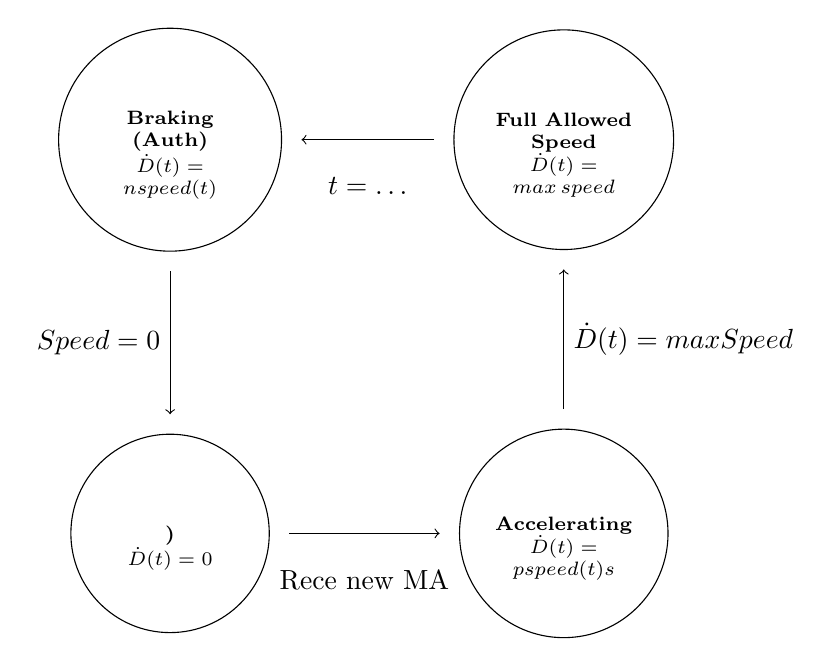
\begin{tikzpicture}[node distance = 3cm]

\tikzstyle{box1}=[circle, draw, text width = 2cm, font=\scriptsize]
\tikzstyle{box3}=[rectangle, draw, text width = 2cm, font=\scriptsize]
\tikzstyle{arrow}=[->,shorten >=7pt,shorten <=7pt]
\tikzstyle{biarrow}=[<->,very thick,shorten >=7pt,shorten <=7pt]


\node (A) [box1]  at (0,0)                  {\begin{center} \textbf{)} \\
							$\dot{D}(t) = 0$  \end{center}

                                            };

\node (B) [box1]    at (5,0)          {\begin{center} \textbf{Accelerating} \\
       $\dot{D}(t) = pspeed(t)s$  \end{center}

};

\node (C)[box1] at (0, 5)  { \begin{center} \textbf{Braking (Auth)}\\
					                   $\dot{D}(t) = nspeed(t)$ \end{center}
                                               
						};

\node (D)[box1] at (5, 5)  { \begin{center} \textbf{Full Allowed Speed }\\
					                   $\dot{D}(t) = max\, speed$ \end{center}
                                               
						};


\draw [arrow] (B) -- node[right] {$\dot{D}(t) = max Speed$} (D);
\draw [arrow] (A) -- node[below = 10pt] {Rece new MA} (B);
\draw [arrow] (D) --  node[below = 10pt] {$t = \ldots$} (C);
\draw [arrow] (C) -- node [left] {$Speed = 0$} (A);


\end{tikzpicture} 
\end{center}

\label{fig:TrainAuton}
\end{figure}
\end{comment}



\begin{mydef}[Radio Block Controller Hybrid Automaton]

We define a hybrid automaton $H_{RBC}$ as follows:
\begin{description}
\item[Variables] The state of the radio block controller automaton consists of $\underbrace{MA_1, Pos_1, MA_2, Pos_2}_\text{0, \ldots , 249}$, \newline $\underbrace{LastTrain}_{\mathbb{N}}$.

\item[Control Graph] The control graph of the radio block controller automaton consists of four control modes $\{Idle, \, Ready \, to \, Request, \, Wait, \, Granted \}$.

\item[Initial, invariant and flow conditions] \hspace*{0mm}
	\begin{itemize}
	\item $init(Idle) :=   \ldots $

	\end{itemize}

\item[Jump Conditions] \hspace*{0mm}

	\begin{itemize}
	\item $jump(Ready to Request \to Ready to Request) := Train.x.Pos.y \wedge MA.x = y$
	\item $jump(Wait \to Wait) := Train.x.Pos.y \wedge MA.x = y$
	\item $jump(Granted \to Granted) := Train.x.Pos.y \wedge MA.x = y$

	\item $jump(Idle \to Ready to Request) := MA.Req.x \wedge LastTrain = x$
	\item $jump(Ready to Request \to Wait) := Req.NextTrack(y)$
	\item $jump(Wait \to Ready to Request) := Deny.LastTrain$
	\item $jump(Wait \to Granted) := Grant.LastTrain$
	\item $jump(Granted \to Idle) := MA.x.EndOf(z)$



	\end{itemize}

\item[Events] \hspace*{0mm}
\begin{itemize}
\item $jump(Ready to Request \to Ready to Request) := Train.x.Pos.y$
	\item $jump(Wait \to Wait) := Train.x.Pos.y$
	\item $jump(Granted \to Granted) := Train.x.Pos.y $

	\item $jump(Idle \to Ready to Request) := MA.Req.x $
	\item $jump(Ready to Request \to Wait) := Req.NextTrack(y)$
	\item $jump(Wait \to Ready to Request) := Deny.LastTrain$
	\item $jump(Wait \to Granted) := Grant.LastTrain$
	\item $jump(Granted \to Idle) := MA.x.EndOf(z)$
\end{itemize}

\end{description}

\end{mydef}



\begin{figure} [h!]

\begin{center}
\begin{tikzpicture}[node distance = 1cm]

\tikzstyle{box1}=[circle, draw, text width = 2cm ]
\tikzstyle{box3}=[rectangle, draw, text width = 2cm, font=\scriptsize]
\tikzstyle{arrow}=[->,shorten >=7pt,shorten <= 7pt]
\tikzstyle{biarrow}=[<->,very thick,shorten >=7pt,shorten <=7pt]


\node (A) [box1]  at (0,0)                  {\begin{center} \textbf{Idle} \\
\end{center}};

\node (B) [box1]    at (7.5,0)          {\begin{center} \textbf{Ready to Request} \\
 \end{center}

};

\node (C)[box1] at (0, 7.5)  { \begin{center} \textbf{Granted}\\
					                \end{center}
                                               
						};

\node (D)[box1] at (7.5, 7.5)  { \begin{center} \textbf{Wait}\\
				
                                                            \end{center}
                                               
						};


\draw [arrow] (B)  .. controls +(0.5cm,  1.5 cm) and +(0.5cm,  -1.5 cm ) .. node[right] {$Req.NextTrack(y)$} (D);
\draw [arrow] (D) .. controls +(-0.5cm,  -1.5cm) and +(-0.5cm, 1.5 cm ) ..   node [left] {$Deny.LastTrain$} (B);
\draw [arrow] (A) -- node[below = 10pt, text width = 4cm] {\begin{center}$MA.Req.x$ \\ $LastTrain = x$\end{center}} (B);
\draw [arrow] (D) --  node[above = 10pt,text width=4cm] {\begin{center}$Grant.LastTrain$\end{center}} (C);
\draw [arrow] (C) -- node [left] {$MA.x.EndOf(z)$} (A);

\draw [arrow] (C) .. controls +(-2cm,  2cm) and +(-2cm, 0.5 cm ) ..   node [above = 5pt, text width = 4cm] {\begin{center}$Train.x.Pos.y$\\ MA.x = y\end{center}} (C);
\draw [arrow] (D) .. controls +(2cm,  2cm) and +(2cm, 0.5 cm ) ..   node [above = 5pt, text width = 4cm] {\begin{center}$Train.x.Pos.y$\\ MA.x = y\end{center}} (D);
\draw [arrow] (B) .. controls +(2cm,  -2cm) and +(2cm, -0.5 cm ) ..   node [below = 6pt, text width = 4cm] {\begin{center}$Train.x.Pos.y$\\ MA.x = y\end{center}} (B);

\end{tikzpicture} 
\end{center}

\label{fig:RBCAuton}
\end{figure}






Safety conditions for the combined system can be separated into discrete and continuous parts.  If we want to specify a safety condition which states that it is not possible for two trains to collide in our current system this could have the following components. 

 the continuous part would state that any movement authority issued by the radio block processor would respect the interlockings separation policy. The discrete part would basically state that there is at least two free track circuits in-between each train.


We will now attempt to formalise the safety condition "The train will always break on time".  What this means formally is that starting from the stop mode whenever the train is in the stop start $D(t) \leq EoA$ Assuming we are in the stop mode and the we receive a movement authority with $EoA > D(t)$. Then we move to the accelerating state in this case we shall perform a case distinct on whether we reach the braking point i.e. $D(t) = BD(EoA, speed)$ or we reach maxspeed.




\begin{mytheorem}
Given a live transition system $(S^t_{H_{T}},  L^{t}_{H_T}) $

 $$\forall \langle a_i, q_i \rangle_{i \geq 1} \in L^{t}_{H_T}.  \forall (a_n, (v, [D(t), EoA,Speed,\dot{Speed},TID])) \in \langle a_i, q_i \rangle_{i \geq 1}$$ $$ \wedge  D(t) \leq BD(EoA,Speed)  \leq EoA$$ 

\begin{proof}


The proof is performed by fixing a trace $ \langle a_i, q_i \rangle_{i \geq 1}$ and  a label/state pair $(a_n, q_n)$ in the timed trace in which the property holds and then proving that for all possible successor label/state pairs $(a_{n+1},q_{n+1})$. Where  the state $q_n = (v, [D(t), EoA,Speed,\dot{Speed},TID])$ and $q_{n+1} = (v', [D(t)', EoA',Speed',\dot{Speed}',TID'])$ 

There are 4 cases for $v$ in which we must argue that the transition $q_n \xrightarrow{a_{n+1}} q_{n+1}$  maintains the property $D(t) \leq EOA$. We further divide each other these cases 
into two sub cases  in which the duration of the transition  $\delta = 0$ or $\delta \in \mathbb{R}_{>0}$



\begin{description}
\item[v = Stop] All possible transitions from the stop mode have a duration $\delta = 0$. There is one possible event that $MA.TID.y$ which will grant a new movement authority $y$ such that $EoA < y$ and cause a jump to the $Accelerating$ mode with $D(t)' \leq BD(y,Speed') < y$


\item[v = Accelerating] In the case that the duration of the transition $\delta = 0$ and the successor state is $q_{n+1} = (Braking,[D(t)' = D(t), EoA' = EoA,Speed' = Speed ,\dot{Speed}' = \dot{Speed},TID' = TID]$ and either $D(t) = BD(EoA,Speed)$ or $Speed = MaxSpeed$ has occurred. If $D(t) = BD(EoA,Speed)$ then $D(t)' = BD(EoA', Speed') \leq EoA'$. The other case that $Speed = MaxSpeed$, $v' = Full \,  Allowed \, Speed$ and $D(t)' \leq BD(EoA', Speed') \leq EoA'$. If the successor state and the current state are the same then an event has occurred and $D(t) \leq BD(EoA,Speed) < $.
  
In the case that $\delta \in \mathbb{R}_{< 0}$



 In the $Accelerating$ mode we have $\dot{Speed} = 1$ with $D(t) \leq BD(Speed, t_1) \leq  EoA$. There are two cases either $D(t) = BD(Speed,t_1)$ or $D(t) < BD(Speed, t_1)$.  In the case that $D(t) = BD(Speed,t_1)$  a jump occurs taking the system into the Braking mode
with $D(t_1) = BD(Speed,t_1) < EoA$. In the case that $D(t_1) < BD(Speed,t_1)$ time will progress and at some point in the future $t_2$ the train will with reach the braking point $D(t_2) = BD(Speed',t_2)$ or $Speed' = Max Speed \wedge (D(t_2) < BD(Speed', t_2)$.   In the case that $D(t_2) = BD(Speed', t_2)$ a jump will occur taking the train into the braking mode with $D(t_2) = BD(Speed',t_2) < EoA$. Otherwise $Speed = MaxSpeed$ and a jump is performed to the $Full Allowed Speed$ mode with $D(t_2) < BD(Speed', t_2) < EoA$.

\item[v = Full Allowed Speed] In the $Full Allowed Speed$ mode have  two cases  $D(t) = BD(Speed, t)$ with $t = t_1$ or $t_2$,  $t_1 < t_2$. In the first case a jump occurs instantaneously to the $Braking$ mode with $D(t_1) = BD(Speed, t_1) < EoA$ In the second case time elapses to a point in the future $t_2$ and $D(t)$ increases until $D(t_2) = BD(Speed, t_2)$  then the system will perform a jump to the $Braking$ mode with $D(t_2) = BD(Speed, t_2)  < EoA$. 

\item[v = Braking] In the Braking mode there are two cases either $MA.TID.y \wedge Speed > 0$ or $Speed = 0$. Since the train is braking by the definition of $BD$,  $D(t_2) \leq BD(Speed,t_2)$ will continue to hold for any amount of time in this state.  In the case that $MA.TID.y \wedge Speed > 0$ we receive a new movement authority $y$ with $y < EoA$ and a jump is performed to the $Accelerating$ mode with $D(t_2) \leq BD(Speed', t_2) < y$. In the case that $Speed = 0$ a jump occurs to the $Stopped$ state.
\end{description}


\begin{comment}
Initially we are in the stop state and have $D(t) \leq EOA$. There is only one possible transition from this state. we receive a new movement authority with $D(t) < EOA$ and proceed to the accelerating state.
We have two possible cases from the accelerating state. The first case is that the train reaches the braking point and enters the braking state $D(t) = BD(t,speed)$. In this case the trains speed speed will decrease by -1 per unit of time and the train will enter the stop state $EOA$.
The second case is that the train reaches max speed and goes into the maxspeed state. If the train reaches $D(t) = BD(t,speed)$ whilst in the maxspeed state then the train will go into the braking state and the same argument holds from the previous case.
\end{comment}
\end{proof}

\end{mytheorem}


Another interesting property of our model is that alone the model of the interlocking allows for "jumping trains" i.e. it allows for track circuits to become free and occupied in a way that does not model the normal movement of trains.
However when the interlocking automaton is placed in parallel with a train automaton it behaves in a

\begin{mytheorem}

In the composite automaton $H_{IL}|| H_{T} $  the event $t_x.t_{x+1}$ will only occur if  and only if$t_x$ is currently occupied in which case $t_x'$ = free and $t_{x+1}' = occupied$.


\begin{proof}
We have to prove the two directions of the statement.

If the 





Assume a train is in $t_x$ and $((x-1) mod 5) * 500 \leq D(t) < x *500$.

There are two cases
\begin{enumerate}
\item If the train is in the Stopped state then a $t_{x}.t_{x+1}$ event will never occur as it is not possible in this state.

\item The train is moving i.e. it is in either of the $Accelerating, \, Braking , \,  Full \, Allowed \, Speed$ states. In this case the position of the train will be increasing and eventually it will happen that $D(t)  mod 500 = 0$. When since $D(t) mod 500 = 0$  satisfies the jump condition the event
 $t_{x}.t_{x+ 1}$ will occur.  
 

\end{enumerate}
\end{proof}
\end{mytheorem}


\section{Maude}
In the following section we shall describe the Maude tool and specifications. 
\subsection{Maude Specifications}

A Maude specification consists of \emph{functional modules} declared using \texttt{fmod} and \texttt{endfm} which contain the following:

\medskip
\begin{center}
\begin{tabular}{| c | l |}
\hline
sorts    & \texttt{sort} $s$ or \texttt{sorts}  $s \ s' .$ \\ \hline
subsorts  & \texttt{subsort} $s < s' \ .$ \\ \hline
function symbols  & \texttt{op} $f \ :  \ s_1 \ldots s_n$ \texttt{->} $s \ .$ \\ \hline
variables  & \texttt{vars} $v \ v' : s' .$\\ \hline
uncondition equations  &\texttt{eq} $t = t' .$\\ \hline
condition equations & \texttt{ceq} t = t' \texttt{if} $cond$ \\ \hline
membership axioms & \texttt{mb} $t \ : \ s \ .$ or \texttt{cmb} $t  \ : \ s$ \texttt{if} $cond \ .$  \\ \hline
\end{tabular}
\end{center}

%%% Read the Maude papers as this is currently very close to the description of a maude specification found in the RT maude theory paper.

Formally a Maude specification is a \emph{rewrite theory} of the form $\mathfrak{R}=(\Sigma,E,L,R)$, where 

$$ [l] : t \to t' \mathbf{if} \bigwedge^{n}_{i = 1} u_i \to v_i \bigwedge^{m}_{j = 1} w_j = w'_j $$

where $l$ is a label $l \in L$ and $t$, $t'$, $u_i$, $v_i$, $w_j$ and $w'_j$ are implicitly universally quantified variables representing $\Sigma$-terms. Maude theories are \emph{order-sorted} allowing for the specification of subsorts which is achieved by including into the specification a partial order relation over sorts. Given two sorts $s$ and $s'$ this partial order relation $s \leq s'$ is interpretted as subset inclusion $A_s \subseteq A_{s'}$ in a model $A$.


\begin{mydef}[Rewrite Theory]


\end{mydef}

\subsubsection{Example Maude Specification}
The following is a specification of the natural numbers in Maude:

\begin{verbatim}
fmod BASIC-NAT is
        sort Nat .

        op 0 : -> Nat .
        op s : Nat -> Nat .
        op _+_ : Nat Nat -> Nat .

        vars N M : Nat .

        eq 0 + N = N .
        eq s(M) + N = s(M + N) .
endfm
\end{verbatim}



\section{Real Time Maude}
One extension of Maude that has been used to model and verify hybrid systems is Real Time Maude. There is an example of a distributed sensor network that has been modelled and verified using this tool.
\subsection{Real Time Maude Specifications}
A Real Timed Maude specification consists of \emph{timed modules} that start with \texttt{tmod} and end with \texttt{endtm}. Formally a Real Time Maude specification is a real-time rewrite theory which can be thought of as a rewrite theory with an interpretation for the abstract time domain together with rewrite rules for terms of type \texttt{System} that have a time duration \cite{PO02}. These rewrite rules can be seperated into two categories, the \emph{tick} rules have a non-zero time elapse and the \emph{instantaneous} rules have a time elapse of zero.

The interpretation of the abstract time domain is mapped to a concrete specification of time during the specification process. Real time Maude comes with two of these specifications as standard the most simple  is discrete time based on the natural numbers and the more complicated of the two is dense time based on the rational numbers. We shall use discrete time during the specification as it allows for the best results during the verification process.

\begin{mydef}[Equational Theory Morphism]
 We define an \emph{equational theory morphism} $H: (\Sigma,E) \to (\Sigma', E')$ to consist of the following
\begin{itemize}
\item a monotone map $H:sorts(\Sigma) \to sorts(\Sigma')$ which maps  sorts in $\Sigma$  to sorts in $\Sigma'$

\item a mapping which maps every function symbol $f : s_1 \ldots s_n \to s$ in $\Sigma$ to some term $H(f_{s_1 \ldots s_n, s})$ from $\Sigma'$ of sort $H(s)$ such that the following conditions are satisfied:
\begin{enumerate}

\item  $\var{H(f_{s_1 \ldots s_n, s})} \subseteq {x_1:H(s_1), \ldots, x_n:H(s_n)}$

\item if the operator $f: s_1 \ldots s_n \to s$ can be subsort overloaded $f: s'_1 \ldots s'_n \to s'$ such that $s_i \leq s'_i, s\leq s'$ then it is possible to substute each variable $x_i:H(s'_i)$ by the corresponding variable $x_i:H(s_i)$ in the term $H(f_{s'_1 \ldots s'_n, s})$ and obtain $H(f_{s_1 \ldots s_n, s})$.

\item For every axiom: $$(\forall y_1:s_1, \ldots y_k : s_k) u = v \ \textbf{if} \ C$$ in E the homomorphic extension of $H^*$ to terms and equations in the condition $C$ causes the following to hold:
   $$E' \models (\forall y_1 : H(s_1), \ldots, y_k : H(s_k)) H^*(u) = H^*(v) \ \textbf{if} \ H^*(C)$$

\end{enumerate}

\end{itemize}

\end{mydef}

\begin{mydef}[Real-Time Rewrite Theory]
We define a \emph{real-time rewrite theory} $\mathfrak{R}_{\phi,\tau}$ to be a tuple $(\mathfrak{R}, \phi,\tau)$ containing a rewrite theory $\mathfrak{R} = (\Sigma, E,L,R) $ where:

\begin{itemize}
\item $\phi$ is an equational theory morphism $\phi : \mathit{Time} \to (\Sigma, E)$ that maps objects in the theory \textit{Time} to objects in the equational theory $(\Sigma , E)$.

\item The time domain is functional i.e. if a term $r$ of sort $\phi(Time)$  has a rewrite proof $\alpha: r \to r'$ then $r = r'$ and the identity proof of $r$ is equivalent to $\alpha$.

\item There is a designated sort typically called \textit{State} and a sort \textit{System}, contained within $(\Sigma, E)$, which has no supersorts or subsorts and only one operator that does not satisfy any non trivial equations:

$$\{\_\}: State \to System$$

Further to this condition, it is all required that the sort \textit{System} does not appear in $s_1, \ldots s_n$ the domain  of  any operator $f: s_1, \ldots s_n$.

\item For each rewrite rule with $u$ and $u'$ of sort \textit{System} in $\mathfrak{R}$ of the following form\footnote{All other rules which are not of this form are called \emph{local} rules and have an instantaneous zero time elapse. These do not act on the system as a whole but rather on one or more of its components.}:

there is an assigned term $\tau_l(x_1 \ldots x_n)$ of sort $\phi(Time)$ within $\tau$.

\end{itemize}
\end{mydef}
 
\subsubsection*{Example Real Time Maude Specification}
The following a very simple model of a train Real Time Maude that moves one unit of distance in one time unit along a circular track of length 500. It defines a sort \texttt{TrainState} and a single state \texttt{move}. We have a constructor train of type \texttt{System} which consists of a train state and a natural number.  


\begin{verbatim}
(tmod DISCRETE-SINGLE-TRAIN is protecting NAT-TIME-DOMAIN .
  sort TrainState .
  ops  move :  -> TrainState [ctor] .
  op train : TrainState Nat -> System [ctor] .
 
  vars N : Time .
  crl [travel] : {train(move,N)} => {train(move,N + 1)} in time 1 if N < 500 .
  rl [reset] : {train(move,500)} => {train(move,0)} . 
         
endtm)
\end{verbatim}

\subsubsection*{Executing a Real Time Maude Specification}
Real Time Maude allows one to execute or simulate a real time system by applying rewriting rules to a term of type \texttt{System}.
The command \texttt{(trew \{System\} in time <= t)} will attempt to rewrite the system to a state $t$ time units in the future. This isnt always possible though as the system may deadlock. The following command attempts to rewrite a train, which initially has distince $0$, to its state in 100 units of time in the future: 
\begin{center}
\texttt{(trew {train(move,0)} in time <= 100 .)}
\end{center}

The result from this timed rewrite is as follows:
\begin{verbatim}
rewrites: 4027 in 4ms cpu (3ms real) (1006750 rewrites/second)

Timed rewrite  {train(move,0)} in DISCRETE-SINGLE-TRAIN 
with mode deterministic time increase in time <= 100

Result ClockedSystem :
  {train(move,100)} in time 100
\end{verbatim}


\subsection{Object Orientated Specification in Real Time Maude}
Real Time Maude is based on Full Maude which contains message and object constructs for object orientated specification. Using these constructs its possible to model ERTMS as several synchronously communicating processes. A Real Time Maude specification consists of  \emph{timed object orientated modules} which start with \texttt{tomod} and end with \texttt{endtom}.
\medskip
We can define the following:
\begin{align*}
\textbf{classes}: & \texttt{ class C | a1 : ⟨Sort-1⟩, ... , an : ⟨Sort-n⟩ . } \\
\textbf{objects}: & \texttt{ < O : C | a1 : v1, ... , an : vn >  . } 
\end{align*}
where $C$ is the class identifier $O$ is the object name  $a_1 \ldots a_n$ are attribute names and $v_1 \ldots v_n$ are values. \\
\medskip
To model communicating processes Real Time Maude uses a messages construct.
\begin{center}
\verb|msgs M1 ... Mn : Sort-1 ... Sort-n -> Msg . | 
\end{center}


\subsubsection*{Configurations in Real Time Maude}
Objects and messages in a specification are given a sort of \texttt{Configuration} which is a subsort of type \texttt{System}. The composition operation for these configuration allows for a combination of objects and messages to form new configurations. This composition operation is also commutative meaning the order of messages and objects in any configuration is ignored. This allows for more generalised writing rules in an object orientated specification that speak about specific objects and messages that are part of some bigger configuration that does not affect the firing of the rule.

\begin{verbatim}
mod CONFIGURATION is  
    *** basic object system sorts  
    sorts Object Msg Configuration .  
 
    *** construction of configurations  
    subsort Object Msg < Configuration .  
    op none : -> Configuration [ctor] .  
    op __ : Configuration Configuration -> Configuration  
         [ctor config assoc comm id: none] .
\end{verbatim}



\subsubsection*{Example Object Orientated Specification}
The following is an example consisting of two classes of object which serves to demonstrate some of the advantages of object orientated specification as well as some of the pit falls. Firstly there is the class defining D objects which count modulo 500 and transmit a message containing the current count. Secondly there is class defining a object B that reads messages from a D object. 

\begin{verbatim}
(tomod EXAMPLE1 is protecting NAT-TIME-DOMAIN .
  msgs msgD  : Nat -> Msg .  
  class  D | d : Nat .
  class  B | b : Nat .
  vars N: Nat .
  var O : Oid .
  var REST : Configuration .
 
  rl [makeD] : {< O : D | d : N > REST} => 
  {msgD(N + 1 rem 500)  
  < O : D | d : (N + 1) rem 500 > REST} in time 1 . 

  rl [readB] : {msgD(N) < O : B | > REST} => 
  {< O : B | b : N > REST}  . 
endtom)
\end{verbatim}

We can execute the specification as follows:
\begin{center}
\texttt{(trew {< myD : D | d : 0 > < myB : B | b : 0 >} in time <= 2 .)}
\end{center}

Resulting in the following output:
\begin{verbatim}
rewrites: 6246 in 7ms cpu (7ms real) 
(805000 rewrites/second)

Timed rewrite  {< myD : D | d : 0 > < myB : B | b : 0 >} 
in EXAMPLE1 with mode deterministic time 
increase in time <= 2

Result ClockedSystem :
  {< myB : B | b : 2 > < myD : D | d : 2 >} in time 2
\end{verbatim}

The following are some states reachable in time 2.

\begin{verbatim}
{< myB : B | b : 1 > < myD : D | d : 2 >}
{< myB : B | b : 2 > < myD : D | d : 2 >}
{msgD(1)< myB : B | b : 2 > < myD : D | d : 2 >}
{msgD(1)msgD(2)< myB : B | b : 0 > < myD : D | d : 2 >}
{msgD(2)< myB : B | b : 1 > < myD : D | d : 2 >}
\end{verbatim}

\emph{Non-determinism} should be avoided unless it is really is a property you want in a model. One way to remove some of these reachable states is to make the variable \texttt{REST} of sort \texttt{ObjectConfiguration}. This forces objects of the B class to read messages after each incrementation of time. If we make this modification to the specification then the following states are reachable in time 2.
\begin{verbatim}
{< myB : B | b : 2 > < myD : D | d : 2 >}
{msgD(2)< myB : B | b : 1 > < myD : D | d : 2 >}
\end{verbatim}


\section{Modelling the European Rail Traffic Management System}
In the following we shall give an overview of the specifications used to model the ERTMS system. Following the hybrid automata describe in \ref{} we have defined one class for each of the 3 hybrid automata.
\subsubsection*{Modelling the Transition of Time}
In our previous Real Time Maude specifications we have had a rewrite rules that work on a specific object or state and increment time for the whole system. This presents a problem as we could have two objects that can both increment the time of the global system independently. We need a way of incrementing the time of the whole global system and then distributing this increment of time amongst the objects of the system. To solve this problem we define operator $\delta$ which describes how distributed system evolves with time.
\begin{verbatim}

op delta : Configuration -> Configuration [frozen] . 

var OCREST : ObjectConfiguration .

op delta : Configuration -> Configuration [frozen] . 

rl [timetrans] : {OCREST} => {delta(OCREST)} in time 1 .
rl [delta1] : delta(CON1 CON2) => delta(CON1)delta(CON2) .

\end{verbatim}

\subsubsection*{Modelling Trains}
We shall now describe the specification of trains. We define the Train class to have a state which like our hybrid automata can be in one of 4 possibilities, constant speed, accelerating, stopped and breaking. As well as the state it also has 6 fields of sort Nat representing the distance, speed, acceleration, movement authority,  current track segment and max speed.

\begin{verbatim}
sort TrainState .
ops  cons acc stop break :  -> TrainState [ctor] .

class Train | state : TrainState, dist : Nat, speed : Nat, ac : Nat,  
                               ma : Nat, tseg : Nat , maxspeed : Nat .
\end{verbatim}

We capture the behaviour of trains using a number of instantaneous and tick rewriting rules. The instantaneous rules are used to capture a change of state within a train. For example if the a train is in the cons state distance to the movement authority becomes less than the distance needed to break to zero in the next moment of time one of these rules will fire and cause a state transition. 

We use the following function to compute the breaking distance:

The division operation is based on repeated subtraction and finally taking the floor or the resulting number. When we divide a number by 2 in the breaking function we add 1 to change this to the ceiling of the resulting number. This prevents a situation where we have a distance of 1 from our moment authority but the breaking distance is 0.

\subsubsection*{Modelling the Radio Block Processor}
We define the RBC state as follows:

\begin{verbatim}
sort RBCState .
ops rbcidle ready wait :  -> RBCState [ctor] .
\end{verbatim}

We define the RBC class as follows:

\begin{center}
\texttt{class RBC | state : RBCState, lasttrain : Oid, ma : MapON, pos : MapON , curreq : SetO  .}
\end{center}
We use maps to store the current movement authorities and positions of the various trains. In order to prevent an infinite amount of requests being made to an interlocking we limit the rbc to make one request on behalf of each train to the interlocking.  To do this we use  \texttt{curreq}, a set of oids, to store which trains have had a request made for them at a given moment of time.

An example RBC transition is as follows:
\begin{center}
\texttt{ rl [rbcgrant] : \{grant(N) < O : RBC | state : wait, lasttrain : T1, ma : MAP1  > REST\} => \{ < O : RBC | state : rbcidle, ma : insert(T1,endoftrack(N),MAP1) > grantma(T1, endoftrack(N)) REST\} .
}
\end{center}


\subsubsection*{Modelling the Interlocking}
An interlocking has two states, either it is idle or it has received a request for a movement authority and must respond. We define an Interlockings state in Real Time Maude as follows:

\begin{verbatim}
sort InterState .
ops idle res :  -> InterState [ctor] .
\end{verbatim}
The interlocking class consists of a interlocking state, a request id which stores the current track segment requestions and 5 Booleans which indicate whether or not a track segment is occupied. We define an Interlocking class in Real Time Maude as follows:
\begin{center}  
\texttt{class Inter | state : InterState, reqid : Nat, t0 : Bool , t1 : Bool , t2 : Bool , t3 : Bool , t4 : Bool .}
\end{center}

All of the rewrite rules on Interlocking objects are instantaneous and do not effect the transition of time.  We can split these rules into two types. Firstly there are interlocking rules that deal with a request


Secondly there are several rewriting rules that deal with granting or denying a received request. There is currently a rule for both denying and granting a request for each track segment depending on the value of the boolean variable.
\begin{center}
\texttt{rl [resreq1g] : {< O : Inter | state : res, t1 : false,  reqid : 1 > REST} => {< O : Inter | state : idle > grant(1) REST} .}
\end{center}


\subsection{Simulating the European Rail Traffic Management System Using Real Time Maude}
We will now see how this executable specification can be used to simulate and obtain a better understanding of the modelled system. For this purpose we have written a small Haskell program that takes the output from multiple timed rewrites and plots them as a graph.

In the following we use an example initial state containing two trains one of which is slower (train1) than the other (train2), an interlocking and a radio block processor. The faster train will eventually catch up with the slow train and it waits for that train to clear all successive track segments before proceeding. The trains start at positions on opposing sides of the track with train1 starting at 0 and train2 starting at 50. The RBC and the interlocking are both initialised with the trains in these positions.

The model of ERTMS  in the  is executed using the following command:
\begin{center}
(trew initialstate2 in time <= 10 .)
\end{center}

In the resulting output at time 10 both of the trains have moved a considerable distance and have requested and received new movement authorities.
 
\begin{figure}
\begin{center}
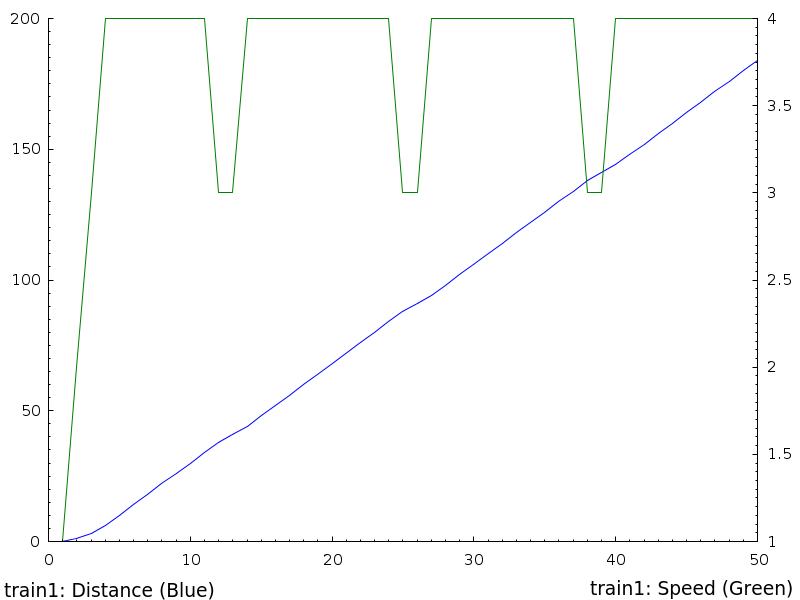
\includegraphics[scale=0.4]{t1graph.png}
\end{center}
\caption{A graph comparing the distance and speed of train1}
\end{figure}

\begin{figure}
\begin{center}
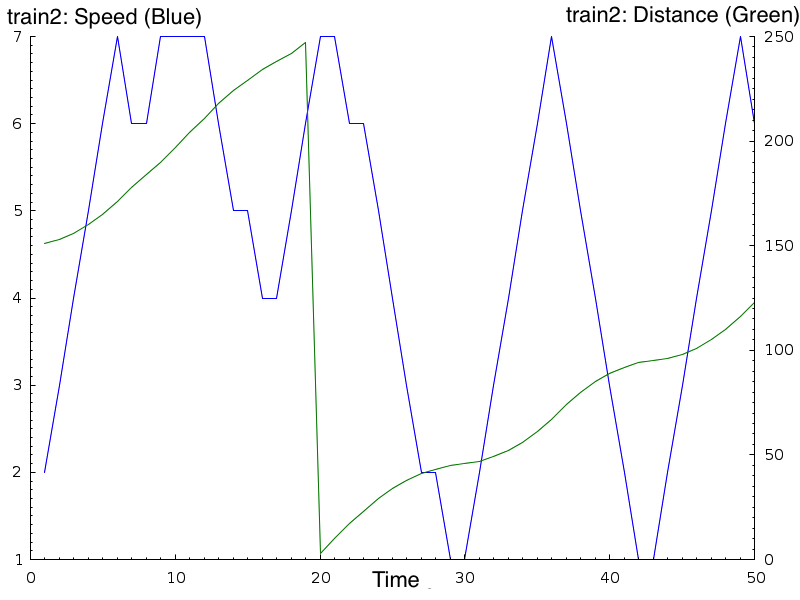
\includegraphics[scale=0.4]{t2graph.png}
\end{center}
\caption{A graph comparing the distance and speed of train2}
\end{figure}

\begin{figure}
\label{t1t2graph}
\begin{center}
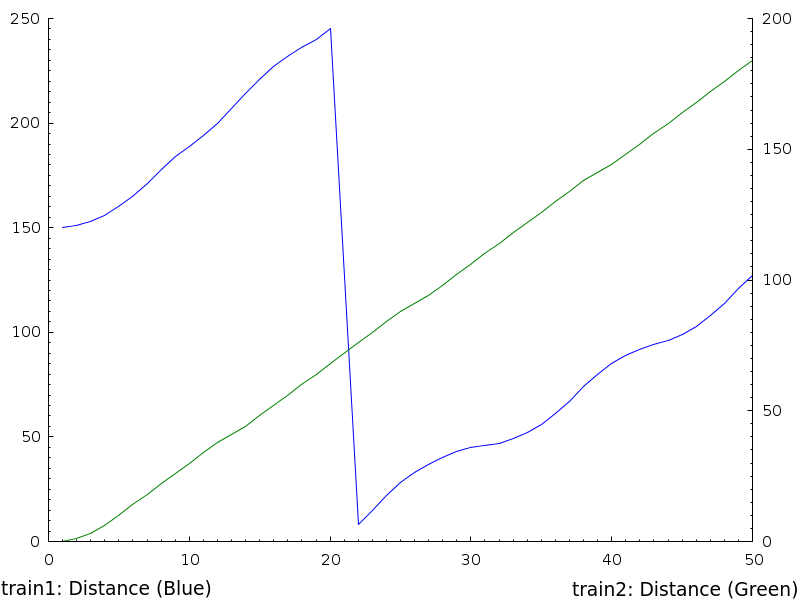
\includegraphics[scale=0.4]{t1t2graph.png}
\end{center}
\caption{A graph comparing the distances of train1 and train2}
\end{figure}

In fig\ref{t1t2} we see that train2 never enters the same track segment as train1.

\section{The Maude Linear Temporal Logic Model Checker}
The Real Time Maude system includes a model checker for linear temporal logic \cite{ES00}. In the following we shall present formal definitions for linear temporal logic and the model checking problem for formulae in this logic.

\subsection{Linear Temporal Logic}
In order to perform model checking over a system we typically need a formal language that allows one to speak about time. We need to be able to formalise sentences such as "the next moment of time" and "all moments in time in the future". One such logic that allows us to formalise these statements is linear temporal logic (LTL)\cite{AP77}. 

\begin{mydef}[Atomic Propositions]
Given a set of symbols $S$ we inductively define the set of atomic propositions AP as follows:
\begin{itemize}
\item If $s$ is in the set of symbols $s \in S$ then $s \in AP$.

\item if $p_1$ is an atomic proposition $p_1 \in AP$ then $\neg p_1 \in AP$.

\item given two atomic propositions $p_1$ and $p_2$ then $p_1 \circ p_2 \in AP$ where $\circ$ is a propositional connective $\circ \in \{ \wedge,\vee,\to \} $.
\end{itemize} 
\end{mydef}

Using these atomic propositions combined with the temporal operators it is possible to define a syntax for temporal logic formulae.

\begin{mydef}[Syntax of Linear Temporal Logic]
Let $AP$ be the set of atomic proposition names then:

\begin{itemize}
\item $\top$ and $\bot$ are well formed formulas.
\item if $p \in AP$ then $p$ is well formed formula (wff).

\item if $f$ and $g$ are wff  then $\star f$ and $f \circ g$ are wffs where $\star \in \{\neg,\mathbf{X},\mathbf{G}, \mathbf{F}\}$ and $\circ \in \{ \wedge,\vee,\textbf{R},\textbf{U} \}$.
\end{itemize}

\end{mydef}
We write $LTL(AP)$ to denote the LTL logic formulas for a given set of atomic propositions $AP$.

LTL operations can be used to speak about paths through a system specified as a Kripke structure.
a \emph{path} $\pi$ is a sequence of states $s_1, \ldots s_n$ and a \emph{path formula} is one that holds in each given state of a path. We define $Path(K,s_0)$ to be the set of paths starting at state $s_0$ in the Kripke structure $K$ as the set of functions $\phi : N \to S$ such that $\phi(0) = a$ and the $\phi(n) \to \phi(n+1)$. 

We shall now look at the semantics of LTL firstly using an informal description of the LTL operations and secondly by giving a formal semantics for LTL. The following is a description of the 5 LTL operations over paths of a Kripke Structure.

\begin{itemize}
\item \textbf{X} $f$ : The property $f$ holds in the \emph{next} moment of time.
\item \textbf{G} $f$ : The property $f$ is \emph{globally} true. i.e. it holds for all times on all paths. 
\item \textbf{F} $f$ : The property $f$ is \emph{finally} true. i.e. there exists a time such that the property $f$ holds on a path.
\item $f$ \textbf{U} $g$ : For all paths the property globally $f$ holds \emph{until} property $g$ holds. 
\item $f$ \textbf{R} $g$ : f holds up to and including the point when $g$ holds.
\end{itemize}

%%%
%%% We need to formalise the following definition. Semantics of Linear Temporal Logic Formula?
%%% 
\begin{mydef}[Semantics of Linear Temporal Logic]
We define the semantics of a linear temporal logic formula $\phi \in LTL(AP)$ in terms of a satisfaction relation $$K,s \models \phi$$ over a Kripke structure $K = (S,T,L)$ and a state $s \in S$ as follows:

$$K,s \models \phi$$ holds if and only if $\forall \pi \in Path(K, s)$, $K,\pi \models \phi$ holds.

We define what it means for $K, \pi \models \phi$ to hold inductively as follows:

\begin{itemize} 
\item $K,\pi \models \phi$ always holds.

\item For some atomic proposition $p \in AP$ the following always holds:
     $$K,\pi \models p \leftrightarrow p \in L(\pi(0))$$

\item For some LTL formula $\mathbf{X} \phi \in LTL(K)$ the following always holds:
$$ $$

where $succ$ is a successor function $succ: N \_ \to N$ such that $succ;\pi(n) = \pi(succ(n)) = \pi(n + 1)$.

\end{itemize}

\end{mydef}





\section{Model Checking the European Rail Traffic Management System}
In the following section we will demonstrate an approach to apply the Real Time Maude LTL model checker to verify the Real Time Maude specification described previously.
Firstly we shall define the property we want to check in the Real Time Maude system. To do this we have to define a satisfaction relation which describes what it means for the property to hold in a state of the system we are checking.  The property we shall consider in this case is that the moment authorities of two trains in system do not overlap. Logical property we define identifies the individual trains using their object identifiers and then computes whether or not an over lap has occured using a boolean formula.  We shall show that it is possible to verify this property over a time period large enough for all normal behaviours of the system to occur. 

\subsection*{Defining a Satisfaction Relation}
We shall now describe how to define the behaviour of the satisfaction relation for a given system and property as a Real Time Maude specification. The satisfaction relation itself is predefined in a specification as an operation which takes a State and a property which is of type Prop and computes a boolean. Maude defines the satisfaction relation $\models$ in the following module:
\begin{verbatim}
  fmod SATISFACTION is  
    protecting BOOL .  
    sorts State Prop .  
    op _|=_ : State Prop -> Bool [frozen] .  
  endfm
\end{verbatim}
The sorts \texttt{State} and \texttt{Prop} are undefined as is the behaviour of $\models$. It is left to the user of the model checker to define the behaviour for their own purposes.

We can check that a train is in a specific state as follows:
\texttt{ops train-cons : Oid -> Prop [ctor] .} \\ \medskip
\texttt{eq {REST < O1 : Train | state : cons >} |= train-cons(O1') = (O1 == O1') . } \\
\bigskip

We can check that a train has a certain speed as follows:

\texttt{op train-s : Oid Nat -> Prop [ctor] .} \\ \medskip
\texttt{eq {REST < O1 : Train | speed : N1 >} |= train-s(O1',N1') = (N1 == N1') and (O1 == O1') .}

The main movement authority that we want to check is that the movement authorities of two trains does not over lap.
To do this we define a Property nomaoverlap(O1,O2) of type \texttt{Oid Oid -> Prop [ctor]} as follows: 

\begin{center}
\texttt{eq {REST < O1 : Train |  dist : D1 , ma : M1 > < O2 : Train |  dist : D2 , ma : M2 >} |= nomaoverlap(O1',O2') = (O1 == O1') and (O2 == O2') and noolap(D1,M1,D2,M2) .} 
\end{center}

This definition features an external operation which computes a boolean depending on whether a set of inequalities are satisfied. 

\begin{center}
\texttt{eq noolap(D1,M1,D2,M2) = ((D1 < M1) and (M1 < D2) and (D2 < M2)) or ((D2 < M2) and (M2 < D1) and (D1 < M1)) or ((D1 < M1) and (M2 < D1) and (M1 < D2)) or ((D2 < M2) and (M1 < D2) and (M2 < D1) )  .}    
\end{center}

\subsection{Execution of The LTL Model Checker}

The Real Time Maude LTL model checker is then called using the following command:

\begin{center}
\texttt{(mc initialstate2 |=t [] nomaoverlap(train1,train2) in time <= 30 .)}
\end{center}
The command states that we are applying timed model checking to check that it is globally true that the movement authorities of the trains do not over lap at all moments in time less than or equal to 30. This results in the following output from Real Time MAude which indicates that the property was succesfully verified in 3 minutes and 22 seconds.
\begin{verbatim}
rewrites: 138889387 in 179663ms cpu (202024ms real) (773054 rewrites/second)

Model check initialstate2 |=t[]nomaoverlap(train1,train2)in 
MODEL-CHECK-ERTMS8 in time <= 30 with mode deterministic time increase

Result Bool :
  true
\end{verbatim}

Unfortunately the Real Time Maude LTL model checker can not detect the congruence between difference configurations of control system. Therefore the state space is infinite and it is impossible to do untimed model checking on the above model checking problem. It is however possible to do timed model checking within a reasonable time limit that allows for all behaviours of the system to be verified.
